\documentclass[a4paper, 12pt]{article}

\usepackage[utf8]{inputenc}
\usepackage[T1]{fontenc}
\usepackage[spanish]{babel}
\usepackage[margin=1in, top=1in, bottom=1in, includefoot]{geometry}
\usepackage{graphicx}
\usepackage{fancyhdr}
\usepackage{parskip}
\usepackage{helvet}
\usepackage{xcolor}
\usepackage{hyperref}
\renewcommand{\familydefault}{\sfdefault}
\definecolor{light-gray}{gray}{0.95}
\newcommand{\code}[1]{\colorbox{light-gray}{\texttt{#1}}}
\pagestyle{empty}
\hypersetup{
    colorlinks=true,
    linkcolor=blue,
    filecolor=magenta,
    urlcolor=cyan
}

\begin{document}

\section*{Proyecto Archivos}

\subsection*{Funcionamiento del programa}

El proposito de este programa es representar las funciones basicas de una base de datos (agregar, mostrar, modificar 
y eliminar), en Java y utilizando archivos de texto y binarios.
El programa consta de tres clases con los nombres: \textbf{Main}, \textbf{Encriptacion} y \textbf{GestionarArchivos}.
La clase Main sólo consta de un menú que no es mas que un ciclo \code{do while} y la condición \code{switch} en 
la cual cada caso representa un método a ejecutar si dicho caso es seleccionado.

Por parte de la clase Encriptacion tiene como funcionalidad el encriptar, desencriptar y generar llaves seguras para
la ejecución de las funciones anteriormente mencionadas de forma correcta. Esta clase utiliza en su mayoría cuatro otras
clases por parte de Java que son \code{Cipher}, \code{SecureRandom}, \code{SecretKey} y \code{KeyGenerator}, las cuales se
encargan de hacer el proceso de encriptado en conjunto con el algoritmo \hyperref[aes]{AES}.

En la clase GestionarArchivos como su nombre lo indica se encarga de crear y eliminar archivos dependiendo del método
que se haya escogido en el menú. Dichos métodos a su vez se encuentran en esta clase, estos son: 

\begin{itemize}
  \item \code{agregarCuentas}
  \item \code{mostrarCuentas}
  \item \code{modificarCuentas}
  \item \code{eliminarCuentas}
  \item \code{pedirDatos}.
\end{itemize}

\subsection*{Conceptos nuevos}

\subsubsection*{Try-Catch}
\code{try - catch} es un mecanismo para poder capturar errores que ocurren en la ejecución del programa, y así tener un programa
más tolerante a fallas y errores.

\subsubsection*{Throws}
\code{throws} es la forma en Java de lanzar un excepcion (cualquiera) dentro de un método, para código posible a fallar
o dar error durante la ejecución, por lo que al ser utilizado en métodos, este debe estar en la firma del mismo.

\subsubsection*{Runnable}

\subsection*{Encriptación AES (Advanced Encryption
Standard)}\label{aes}

Como todos los métodos de encriptación, el AES convierte el texto sin
formato en un código que sólo puede descifrar quien tenga la clave.

\textbf{AES} tiene un tamaño fijo de bloque de 128 bits y tamaños de
clave de 128, 192 y 256 bits. Este opera en una matriz de 4x4
\textbf{bytes} llamada \emph{state}.

\subsubsection*{Tipos de AES}\label{tipos-de-aes}

\begin{itemize}
\item
  \textbf{AES-128}: este método utiliza una longitud de clave de 128 bits para el
  cifrado y el descifrado, lo que da lugar a 10 series de cifrado con
  3,4 x 1038 combinaciones potenciales diferentes.
\item
  \textbf{AES-192}: este método utiliza una longitud de clave de 192 bits para
  cifrar y descifrar, lo que da lugar a 12 series de cifrado con 6,2 x
  1057 combinaciones potenciales diferentes.
\item
  \textbf{AES-256}: este método utiliza una longitud de clave de 256 bits para
  cifrar y descifrar, lo que da como resultado 14 series de cifrado con
  1,1 x 1077 combinaciones potenciales diferentes.
\end{itemize}

\subsubsection*{Pasos del sistema AES}\label{pasos-del-sistema-aes}

\begin{enumerate}
\def\labelenumi{\arabic{enumi}.}

\item \textbf{Inicialización de claves}: Primero, se selecciona una clave de cifrado de longitud adecuada (128, 192 o 256 bits). Esta clave se usa tanto para cifrar como para descifrar los datos.

\item \textbf{SubBytes}: Cada byte del bloque de datos se sustituye por otro byte según una tabla de búsqueda (S-Box). Esto confunde los datos y dificulta su análisis.

\begin{center}
  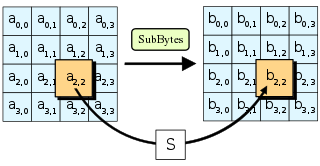
\includegraphics[width=0.4\textwidth]{images/SubBytes.png}
\end{center}

\item \textbf{ShiftRows}: Los bytes en las filas del bloque de datos se desplazan circularmente hacia la izquierda. Esto mezcla los datos y evita patrones predecibles.

\begin{center}
  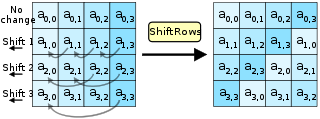
\includegraphics[width=0.4\textwidth]{images/ShiftRows.png}
\end{center}

\item \textbf{MixColumns}: Cada columna del bloque de datos se transforma mediante una operación algebraica. Esto proporciona una difusión adicional de los datos.

\begin{center}
  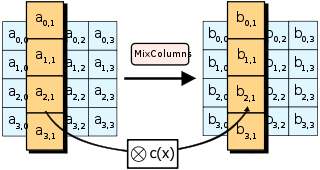
\includegraphics[width=0.4\textwidth]{images/MixColumn.png}
\end{center}

\item \textbf{AddRoundKey}: Se realiza una operación XOR entre el bloque de datos y una subclave derivada de la clave principal para esa ronda. Esto añade una nueva capa de seguridad.

\begin{center}
  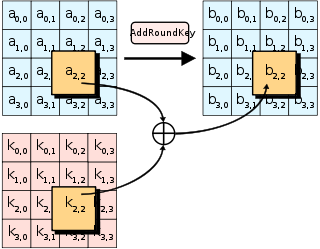
\includegraphics[width=0.4\textwidth]{images/AddRoundKey.png}
\end{center}

\end{enumerate}

El algoritmo AES opera en rondas. Cuantas más rondas, más seguro es el cifrado. El número de rondas depende del tamaño de la clave: 10 rondas para AES-128, 12 rondas para AES-192 y 14 rondas para AES-256. Por lo que estos pasos se realizarán cierta cantidad de veces dependiendo del tamaño de la clave.

\end{document}
